\documentclass[
  manuscript=article,  %% article (default), rescience, data, software, proceedings, poster
  layout=preprint,  %% preprint (for submission) or publish (for publisher only)
  year=20xx,
  volume=x,
]{extra/joas}

% --- blew is the area for authors ---

% remove the following two packages, and delete all \blindtext commands
\usepackage[english]{babel} 
\usepackage{blindtext}
% \usepackage{svg}
\usepackage{algorithm}
\usepackage{algpseudocode}

\usepackage{listings}
\usepackage{xcolor}

\lstset{
    language=Python,
    basicstyle=\ttfamily,
    keywordstyle=\color{blue},
    commentstyle=\color{green!40!black},
    stringstyle=\color{orange},
    showstringspaces=false,
    numbers=left,
    numberstyle=\tiny,
    numbersep=5pt,
    backgroundcolor=\color{gray!10},
    frame=single,
    breaklines=true,
    breakatwhitespace=true,
    captionpos=b
}


% Make sure your article tile is within 12 words
\title{Algebra in Flip Game}

\author{Tang Weihao}
\affiliation{Ningbo University, Ningbo, China}

% maximum five keywords
\keywords{Filp Game; Group Theory; Linear Algebra}


\begin{document}

\begin{abstract}
  This article explores using algebraic methods in the Flip Game, 
  a simple puzzle where the goal is to turn on all lights with minimal steps. 
  It highlights the importance of group theory in abstract algebra and demonstrates how linear algebra, 
  specifically the Gaussian elimination method, can be applied to solve equations in the game. 
  The article showcases how algebraic techniques can be used to analyze game states and operations efficiently.
\end{abstract}


\section{Introduction}

``Filp Game" is a simple and fun mini game. Its basic rules are as follows:

There is a row of N rows and N columns of lights that are all turned off at the beginning. 
When you click on one of the lights, its own state and its upper, lower, left, and right lights (if any) change completely.
It is required to use as few steps as possible to turn on all the lights.

\par Group Theory is a branch of mathematics that studies the properties of groups
 in abstract algebraic structures. 
 A group is an algebraic structure consisting of a set of elements and a binary operation 
 (commonly referred to as ``multiplication").
 Many algebraic structures, such as rings, fields, and modules, 
 can be seen as being formed by adding new operations and axioms on the basis of groups. 
 In addition, the research methods of group theory also have a significant impact on other 
 branches of abstract algebra.

\par In this article, group theory will play a crucial role in exploring the principles in flip games.
 Exploring the mysteries through algebraic methods can provide a good understanding of its essence.


\begin{figure}[ht!]
  \centering
  \begin{minipage}{0.25\textwidth}
    \centering
    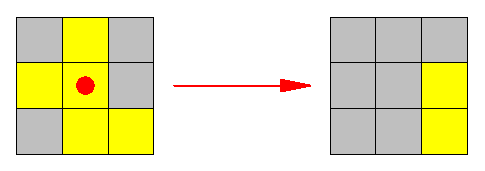
\includegraphics[width=\linewidth]{./flip game/1.eps}
    \caption{Schematic diagram of game}
  \end{minipage}
  \hfill
  \begin{minipage}{0.25\textwidth}
    \centering
    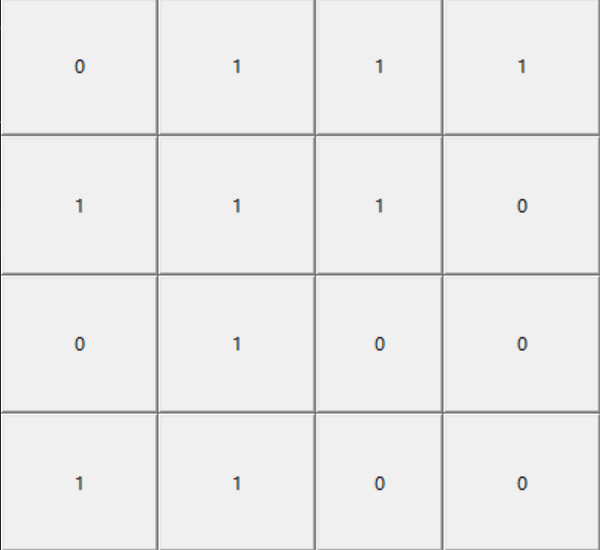
\includegraphics[width=\linewidth]{./flip game/2.png}
  \end{minipage}
  \hfill
  \begin{minipage}{0.25\textwidth}
    \centering
    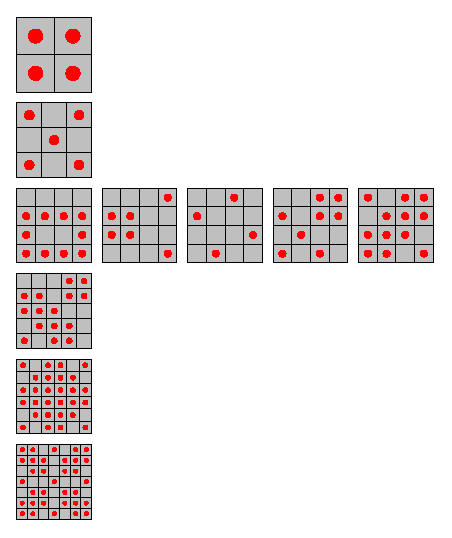
\includegraphics[width=\linewidth]{./flip game/3.eps}
  \end{minipage}
\end{figure}



% \begin{lstlisting}
% def fibonacci(n):
%     a, b = 0, 1
%     for _ in range(n):
%         print(a, end=' ')
%         a, b = b, a + b
%     print()

% fibonacci(10)
% \end{lstlisting}

% \lstinputlisting[language=Python]{./flip game/answer.py}

\newpage
\section{Feature Description}

\subsection{Definition of Group}

If the binary operation on a set  $G \neq\emptyset$
(which is called multiplication of groups, note that it may not necessarily
 be multiplication of numbers in the usual sense, and the result is called \textbf{\emph{product}})
$G\times G \to G$ forms an algebraic structure $(G, \cdot)$ that satisfies:


1. Closure: That is, the operation result of any two elements of $G\cdot$ under $\cdot$ is one element of the set. 
($\forall a, b\in G, a\cdot b \in G$);

2. The law of combination: $\forall a, b, c\in G, (a\cdot b)\cdot c = a\cdot (b\cdot c) $;

3. Unit element (unitary): There is an element $e$ in $G$, so that the result of multiplying any element $a$ in $G$ by 
it (including left and right multiplication) is equal to $a$ itself. 
($\exists e\in G, st. \forall a\in G$, have $ e\cdot a = a\cdot e = a $);

4. Inverse element: $\forall a \in G, \exists b\in G$, st. $a\cdot b = b\cdot a = e$ 
so that the $b$ is called the inverse element of $a$, is denoted as $b=a^{-1}$;

It is called $(G, \cdot)$ a \textbf{\emph{group}}, or a \textbf{\emph{multiplication group}}, abbreviated as $G$.

When there is no ambiguity, $a · b$ can be written as $ab$.

Sometimes, due to contextual reasons, binary operations on a group can also be called \textbf{\emph{addition}} 
(which may not necessarily be the addition of numbers in the usual sense). 
In this case, the operation is usually denoted as $+$, 
the operation of group elements is also denoted as $a + b$, and the group can also be called an \textbf{\emph{addition group}}.



\subsection{The simple situation}

\subsubsection{Symbol Annotation}
For the sake of simplicity and essence, we choose a 3-dimensional case for discussion.
As we can see that the entire state is composed of $3\times 3 = 9$ grids, 
and each grid has only two possible states. Therefore, we can naturally represent each possible 
state using a binary 3-order square matrix of 0 and 1.
\par Then we define $M[3\times 3 |\mod 2]$ as the entire binary matrix with the scale of $3 \times 3$.
Therefore, all the objects we are studying have been fully symbolized.
But it's not enough to depict the connections between the research subjects yet.
To meet the above requirements, 
We can define operations on $M$ based on the characteristics of this model to describe its characteristics.
As obviously we can see that the state of each grid can be changed by a simple and unique operation.
When the state is 1. After this operation, it turns to 0. And vice versa.
Due to this property, we can define the addition $+$ on $M$ as following, which is able to perform this.
\par Define: $+$ \quad $\forall M_1, M_2 \in M$,  $M' = M_1 + M_2$, where $$M'(i, j) = [M_1(i, j) + M_2(i, j)] \mod 2$$
The $M'(i, j)$ means the elements in the i-th row and j-th column of $M'$.


\subsubsection{Basic Analysis}
As mentioned above, we can use $(M, +)$ to describe the system state. Then, we can study the properties of $(M, +)$ and get useful
result for further research.

Firstly, we can prove that $M$ forms an addition group on $+$.
To prove that, we just need to prove it satisfies the 4 rules of group definition.
\par The first closure rule. It's obviously. Adding any two elements still belongs to $M$.
\par The combination rule can be derived from the combination law of regular addition.
\par The Unit element is easy to find. It's the matrix whose element are both 0. We can annotate as $e$.
\par Inverse element. Due to $1 + 1 \equiv 0 + 0 \equiv 0 \mod 2$. We can find that.$\forall M_i \in M$, $M_i$ is the inverse of itself.

\par Therefore, we have proven that it's indeed an addition group. And it's a special group, which satisfies the commutative law
(it can be called additive group, which needs the group is commutative group) and the inverse of each element is its self.


\subsubsection{The structure of group}
We define $u_1 = \begin{bmatrix} 1 & 0 & 0  \\ 0 & 0 & 0  \\ 0 & 0 & 0\end{bmatrix}$, 
$u_2 = \begin{bmatrix} 0 & 1 & 0  \\ 0 & 0 & 0  \\ 0 & 0 & 0\end{bmatrix}$, $\dots$, 
$u_9 = \begin{bmatrix} 0 & 0 & 0  \\ 0 & 0 & 0  \\ 0 & 0 & 1\end{bmatrix}$.
\par That means $u_i$ is the matrix with the i-th element being 1 and the rest being 0.
Obviously, every matrix in $M$ can be expressed uniquely with the $\{ u_i\}_{i=1}^9$.
More precisely, it can be described by set theory as 
$$M = \{ \sum_{i=1}^{9} a_i u_i:\text{$a_i$ = 0 or 1 } \}$$
We can infer that the number of elements in set $M$ is $Card(M) = 2^9 = 512$.
So it is a finite group.
\par In order to further explore its structure, 
We can mimic the above and construct a new linear combination to equivalently represent $M$.
In order to connect with the characteristics of operation between elements, we adopt the following pattern.
\par We define $v_1 = \begin{bmatrix} 1 & 1 & 0  \\ 1 & 0 & 0  \\ 0 & 0 & 0\end{bmatrix}$, 
$v_2 = \begin{bmatrix} 1 & 1 & 1  \\ 0 & 1 & 0  \\ 0 & 0 & 0\end{bmatrix}$, $\dots$, 
$v_9 = \begin{bmatrix} 0 & 0 & 0  \\ 0 & 0 & 1  \\ 0 & 1 & 1\end{bmatrix}$.
\par That means $v_i$ is the matrix where 
the i-th element and its adjacent (distance of 1) elements are 1, and the rest are 0.
The reason we designed this is based on the initial rules: Select the i-th cell and reverse it from adjacent cells.

\par To achieve it, we can find that this is equivalent to add the $v_i$ with the matrix corresponding to previous states.
It means each $\{v_i\}_{i=1}^9$ represent an operation. Due to the commutativity of addition on $M$. 
The order of operations is not important.
\par And we can assert that each operation can occur at most once.
If not, let's assume that the $v_i$ appears more than twice. If the number of occurrences of $v_i$ is odd.
According to commutativity of addition, we can merge $v_i$ at each different position together 
and $v_i$ has a coefficient of an odd. Since it is binary matrices. This is equivalent to a coefficient of 1.
So, the occurrence of more than 1 is redundant and can be omitted.
Similarly, similar conclusions can be drawn in even numbered cases. It's equivalent to not appearing at all.
\par In summary, we can conclude that: The number of operations from one state to another will not exceed 9.

\begin{table}[H]
  \centering
  \small
  \caption{Notation table}
  \label{tb:notation_table}
  \begin{tabular}{lll}
  \toprule
  \textbf{Parameter} & \textbf{Notation} & \textbf{Remarks} \\
  \midrule
  Matrix & $M$ &  entire binary matrix($3\times 3$) \\
  basic matrix & $\{ u_i\}_{i=1}^9$ & A way of constructing $M$ \\
  operative matrix & $\{ v_i\}_{i=1}^9$ & Matrix corresponding to each operation \\
  U space & $U$ & Space composed of $u_i$ \\
  V space & $V$ & Space composed of $v_i$\\
  \bottomrule
  \end{tabular}
\end{table}


\section{Theoretical analysis}

\subsection{Uniqueness of representation}

\paragraph{The Equivalence} We constructed a space earlier that named $V$, which is composed of operation matrices.
The $V$ can be described as $V = \{ \sum_{i=1}^{9} b_i v_i:\text{$b_i$ = 0 or 1 } \}$. 
Obviously, it has $2^9 = 512$ combinations as same as $U$. 
In fact, the $(V, +)$ is also an addition group. It can be simply proven. 
Due to the $M$ represent all the binary matrix, there must have $V\subseteq  M$. 
And $V$ is a subgroup of $M$.
\par As long as we prove that there is only one expression for each element in $V$, 
that is, the element represented by $\{v_i\}_{i=0}^9$ will not be repeated. 
Then, we can obtain that $V = M$. They are completely equivalent. 
Due to it has only finite elements. We can prove that with computer later.

\paragraph{Other Base} As we constructed above, $U$ and $V$ are both the way to rebuild $M$. 
Then we suppose whether there are other bases of similar construction that can achieve this. 
And every element in it can be uniquely expressed. 

\paragraph{The Solution} After analyzing the structure of $M$. 
Let's analyze how to transition from one state to another. That is the solution of the game. 
And we need to analyze the solution of every state and determine the existence of solutions. 
Every solution is written as a vector $x = \begin{bmatrix} b_1 \\ b_2 \\ \vdots \\ b_9 \end{bmatrix}$. 
And we can regard $v_i$ as a number and define $v$ as $v = \begin{bmatrix} v_1 \\ v_2 \\ \vdots \\ v_9 \end{bmatrix}$. 
That means the operations is equivalent to the linear product of $v$ and $x$, $O = x^T\cdot v$.
Finally, obtain a solution system to better describe the structure of the solution. 
To get it, we define $I$ is the matrix of initial state, $T$ is the matrix of target state. 
We assert that if there exists a solution, the necessary and sufficient condition for it is 
$O = I + T = I - T = T - I \in V$. 
Obviously, by the properties of binary, we can simply get $I + T = I - T = T - I$. 
\par $\rightrightarrows$ If there exists a solution. It must be the combination of $\{v_i\}_{i=0}^9$ 
then naturally have the form of $O = x^T\cdot v \in V$.
$\leftleftarrows$ Similarly, if there have $O$ makes $O = T - I \in V$ then it must can be written as 
$O = x^T\cdot v$. So, the $x$ is the solution.



\section{Algorithm implementation}

\paragraph{Equivalence Test} As mentioned earlier, it is necessary to verify that $V$ is another equivalent form of $M$. 
We use Python to solve it. The Python source code is placed at the end. Here is the pseudocode following. 

\begin{algorithm}
  \caption{Pseudocode for the answer function}
  \begin{algorithmic}[1]
  \For{each possible sequence seqs in sequences}
      \State initialize init as org
      \For{each element shun in seqs}
          \State update init by adding bas[shun]
      \EndFor
      \If{init not in st}
          \State add init to st
      \EndIf
  \EndFor
  \State check st for target state tgt
  \If{found}
      \State return the sequence of steps required to transform org into tgt
  \EndIf
  \end{algorithmic}
  \end{algorithm}

The overall idea of this function is to try the possibility of combining all $v_i$, 
and if there are duplicates, remove them. 
In the end, we obtain that the number of elements in $V$ is still $2^9 = 512$, proving that $V=M$. 
Due to we have listed all the situations. If there exists a solution of $I$ and $T$, then it must in the $512$ situations. 
To get the solution, we can also try every situation and find the solution $x$. 

\paragraph{Efficient Of Algorithm} The methods mentioned above exhaust all possibilities and belong to Directly Calculating. 
It is very complex and has a large quantity. Manual calculation is completely impossible. 
Now it's a 3-dimensional situation, which requires $2 ^ 9$ computational resources. 
If we imagine $n$ orders, it would require $2^{n^2}$ calculations. 
This number will be too big to imagine when n is very large. 
We can say that the time complexity of this algorithm is $O(2^{n^2})$. 
This is an exponential time complexity, indicating that this algorithm is very inefficient. 
We usually consider algorithms with polynomial time complexity $O(n^k)$ to be better. 

\paragraph{Linear Algebraic Algorithm}
When we consider the structure of the solution space, we can see the concepts of dimensionality and rank similar to linear spaces. 
So we try to solve problems with linear algebra. To begin with, we write 
$b = \begin{bmatrix} b_1 \\ b_2 \\ \vdots \\ b_9 \end{bmatrix}$, 
$P_i = \begin{bmatrix} v_{i1} \\ v_{i2} \\ \vdots \\ v_{i9} \end{bmatrix}$, this aim to write $v_i$ as a column vector. 
And we define $A = [P_1, P_2, \dots, P_9]$. Then there naturally appears a system of linear equations: $Ax = b$, 
we can regard $b$ as the operation needs to be taken, which is equivalent to $O = T - I$. And the $A$ is the 
matrix which consist of all the basic operations and be written as column vector. What needs to be explained is 
due to the fact that binary systems composed of $0$ and $1$ cannot form a field of numbers, the $M$ and $V$ is not a linear space. 
But we can still solve linear systems of equations through algebraic methods and the $x$ is the solution(if exists). 

\par The Gaussian elimination method is an effective algorithm for solving linear equations, which holds a time complexity of $O(n^3)$. 
Its core idea is to transform the augmented matrix of the linear equation system into a row step matrix 
through a series of elementary row transformations, and then solve the equation system. 
This method can be achieved by constructing an augmented matrix (i.e., adding a constant vector $b$ to the coefficient matrix $A$), 
then transforming the original system into a simpler triangular form through elementary row transformations 
(such as alternating rows, multiplying a certain row by a non negative constant, and adding two rows), 
and finally solving it using a backward substitution algorithm.
\par In our equation, both the matrix $A$, constant vector $b$ and solution $x$ are binary. 
So we need to modify the algorithm before applying. The overall idea reserved, what needs to be changed is 
replacing the regular addition with binary addition during line transformation. Take any two rows $R_1$, $R_2$, 
the result of adding or subtracting the two rows is $R = R_1 + R_2 = R_1 - R_2 = R_2 - R_1$. 

\begin{algorithm}
\caption{Gaussian elimination method}
\begin{algorithmic}
\For{$j$ in range($\text{self.scale}^2$)}
    \State position = [i for i in range($\text{self.scale}^2$) if self.Base[j][i] == 1]
    \State c\_pos = next((f for f in position if f >= j), -1)
    \If{c\_pos == -1}
        \State continue
    \EndIf
    \If{len(position) > 1}
        \For{p in position}
            \If{p != c\_pos}
                \State self.row\_add(c\_pos, p, mode)
            \EndIf
        \EndFor
        \If{c\_pos != j}
            \State self.row\_change(j, c\_pos, mode)
        \EndIf
    \ElsIf{c\_pos != j}
        \State self.row\_change(j, c\_pos, mode)
    \EndIf
\EndFor
\end{algorithmic}
\end{algorithm}

\paragraph{The Result} After completing Gaussian elimination, there are several situations as follows. 
1. Matrix $A$ become a completely stepped shape(all diagonals elements are $1$, the rest are $0$). 
2. There exists diagonals elements which is $0$. 

In situation 1, we can simply get $x$. It equals the transformed $b$, $x = b'$. 
In situation 2, there has still 2 substitution. For the one, If for each element which is 1 in $b'$, 
the corresponding diagonal element of $A$ is also 1. Then the $x = b'$. Else, there is no solution.


\begin{figure}[ht!]
  \centering
  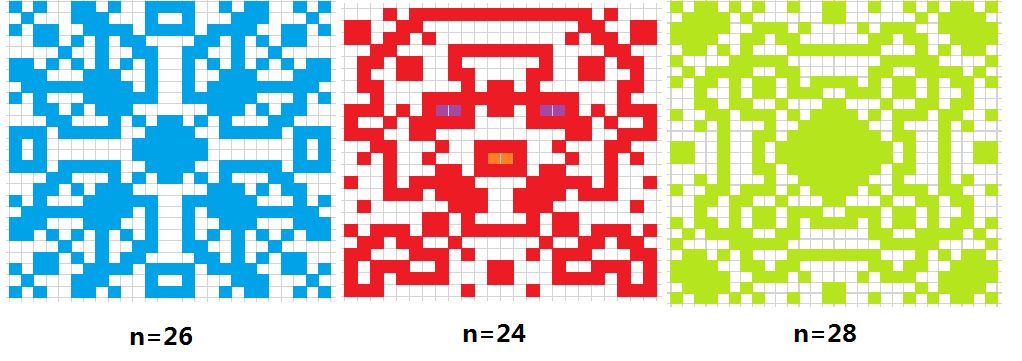
\includegraphics[width=0.45\textwidth]{./flip game/3.png}
  \caption{Implementation of high-order pattern images}
\end{figure}

% \section{Source Code}
% \par Directly Calculating exhaustive algorithm for verifying the structure of solutions:
% \lstinputlisting[language=Python]{./flip game/jgg.py}

% \par A solution algorithm using Gaussian elimination method:
% \lstinputlisting[language=Python]{./flip game/answer.py}


\section{Reference}
\renewcommand{\section}[2]{} 
\begin{thebibliography}{20}

   \bibitem{1} Barile, Margherita. "Lights Out Puzzle." From MathWorld--A Wolfram Web Resource, created by Eric W. Weisstein. https://mathworld.wolfram.com/LightsOutPuzzle.html
   \bibitem{2} Caro, Y. "Simple Proofs to Three Parity Theorems." Ars Combin. 42, 175-180, 1996.
   \bibitem{3} Conlon, M. M.; Falidas, M.; Forde, M. J.; Kennedy, J. W.; McIlwaine, S.; and Stern, J. "Inversion Numbers of Graphs." Graph Th. Notes New York 37, 42-48, 1999.
   \bibitem{4} Cowen, R. and Kennedy, J. "The Lights Out Puzzle." Math. Educ. Res. 9, 28-32, 2000. http://library.wolfram.com/infocenter/Articles/1231/.
   \bibitem{5} Cowen, R.; Hechler, S. H.; Kennedy, J. W.; and Ryba, A. "Inversion and Neighborhood Inversion in Graphs." Graph Th. Notes New York 37, 37-41, 1999.
\end{thebibliography}


\end{document}